% LIST for appendix:
% - distribution of response lengths
% - moral foundations questionnaire


\section{Basic rules on CMV}

\paragraph{Submission rules:}
\begin{enumerate}[A]\singlespacing
\item Explain the reasoning behind your view, not just what that view is (500+ characters required).
\item You must personally hold the view and demonstrate that you are open to it changing.
\item Submission titles must adequately sum up your view and include "CMV:" at the beginning.
\item Posts cannot express a neutral stance, carry a risk of personal endangerment, be self-promotional, or discuss this subreddit (visit r/ideasforcmv instead).
\item Only post if you are willing to have a conversation with those who reply to you, and are available to start doing so within 3 hours of posting.
\end{enumerate}

\paragraph{Comment rules:}
\begin{enumerate}[1]\singlespacing
\item Direct responses to a CMV post must challenge at least one aspect of OP’s stated view (however minor), or ask a clarifying question.
\item Don't be rude or hostile to other users.
\item Refrain from accusing OP or anyone else of being unwilling to change their view.
\item Award a delta if you've acknowledged a change in your view. Do not use deltas for any other purpose.
\item Comments must contribute meaningfully to the conversation.
\end{enumerate}


\clearpage
\section{Moral Foundations Dictionary}

\subsubsection*{Care} amity, benefit*, care, caring, compassion*, defen*, empath*, guard*, peace*, preserve, protect*, safe*, secur*, shelter, shield, sympath*, abandon*, abuse*, annihilate*, attack*, brutal*, cruel*, crush*, damag*, destroy, detriment*, endanger*, exploit, exploited, exploiting, exploits, fight*, harm*, hurt*, impair, kill, killed, killer*, killing, kills, ravage, ruin*, spurn, stomp, suffer*, violen*, war, warl*, warring, wars, wound* 

\subsubsection*{Fairness} balance*, constant, egalitar*, equable, equal*, equity, equivalent, evenness, fair, fair-*, fairly, fairmind*, fairness, fairplay, homologous, honest*, impartial*, justice, justifi*, justness, reasonable, reciproc*, rights, tolerant, unbias*, unprejudice*, bias*, bigot*, discriminat*, dishonest, disproportion*, dissociate, exclud*, exclusion, favoritism, inequitable, injust*, preference, prejud*, segregat*, unequal*, unfair*, unjust*, unscrupulous

\subsubsection*{Loyalty} ally, cadre, cliqu*, cohort, collectiv*, communal, commune*, communis*, communit*, comrad*, devot*, familial, families, family, fellow*, group, guild, homeland*, insider, joint, loyal*, member, nation*, patriot*, segregat*, solidarity, together, unison, unite*, abandon*, apostasy, apostate, betray*, deceiv*, deserted, deserter*, deserting, disloyal*, enem*, foreign*, immigra*, imposter, individual*, jilt*, miscreant, renegade, sequester, spy, terroris*, traitor*, treacher*, treason* 

\subsubsection*{Authority} abide, allegian*, authorit*, bourgeoisie, caste*, class, command, complian*, comply, control, defer, defere*, duti*, duty, father*, hierarch*, honor*, law, lawful*, leader*, legal*, loyal*, mother, mothering, motherl*, mothers, obedien*, obey*, order*, permission, permit, position, preserve, rank*, respect, respected, respectful*, respects, revere*, serve, status*, submi*, supremacy, tradition*, venerat*, agitat*, alienate, apostasy, apostate, betray*, defector, defian*, defy*, denounce, deserted, deserter*, deserting, disloyal*, disobe*, disrespect*, dissent*, dissident, heretic*, illegal*, insubordinat*, insurgent, lawless*, mutinous, nonconformist, obstruct, oppose, protest, rebel*, refuse, remonstrate, riot*, sediti*, subver*, traitor*, treacher*, treason*, unfaithful

\subsubsection*{Sanctity} abstemiousness, abstention, abstinen*, austerity, celiba*, chast*, church*, clean*, decen*, holiness, holy, immaculate, innocent, integrity, limpid, maiden, modesty, piety, pious, preserve, pristine, pure*, purity, refined, sacred*, saint*, steril*, unadulterated, upright, virgin, virginal, virginity, virgins, virtuous, wholesome*, adulter*, apostasy, apostate, blemish, contagio*, debase*, debauche*, defile*, deprav*, desecrat*, dirt*, disease*, disgust*, exploit, exploitat*, exploited, exploiting, exploits, filth*, gross, heretic*, impiety, impious, indecen*, intemperate, lax, lewd*, obscen*, pervert, profan*, profligate, promiscu*, prostitut*, repuls*, ruin*, sick*, sin, sinful*, sinned, sinner*, sinning, sins, slut*, stain*, taint*, tarnish*, tramp, trashy, unchaste, unclean*, wanton, whore, wicked*, wretched*

\subsubsection*{General Morality} bad, blameless, canon, character, commendable, correct, decen*, doctrine, ethic*, evil, exemplary, good, goodness, honest*, ideal*, immoral*, indecen*, integrity, laudable, lawful*, legal*, lesson, moral*, noble, offend*, offensive*, piety, pious, praiseworthy, principle*, proper, righteous*, transgress*, upright, upstanding, value*, wholesome*, wicked*, worth*, wretched*, wrong*

\section{Additional Descriptive Information}
\renewcommand\thefigure{A.\arabic{figure}}
\renewcommand\thetable{A.\arabic{table}}
\setcounter{figure}{0}
\setcounter{table}{0}



\subsection{Distribution of Moral Foundation Proportions in Paired Data}

\begin{figure}[h]
\centering
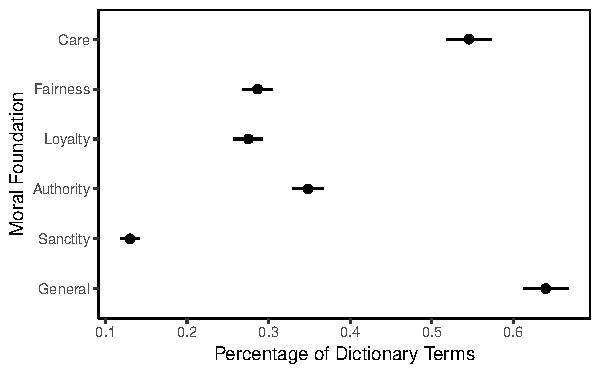
\includegraphics{/data/Dropbox/Uni/Projects/2017/cmv/calc/fig/mft_op_individual.pdf}
\caption[Moral Foundations in Paired Data]{Moral Foundations in Paired Data: Average percentage of dictionary terms relative to the total number of words in each original post starting a discussion (including 95\% confidence intervals).}
\end{figure}


\clearpage
\subsection{Distribution of MFT cosine similarity in Paired Data}

\begin{figure}[h]
\centering
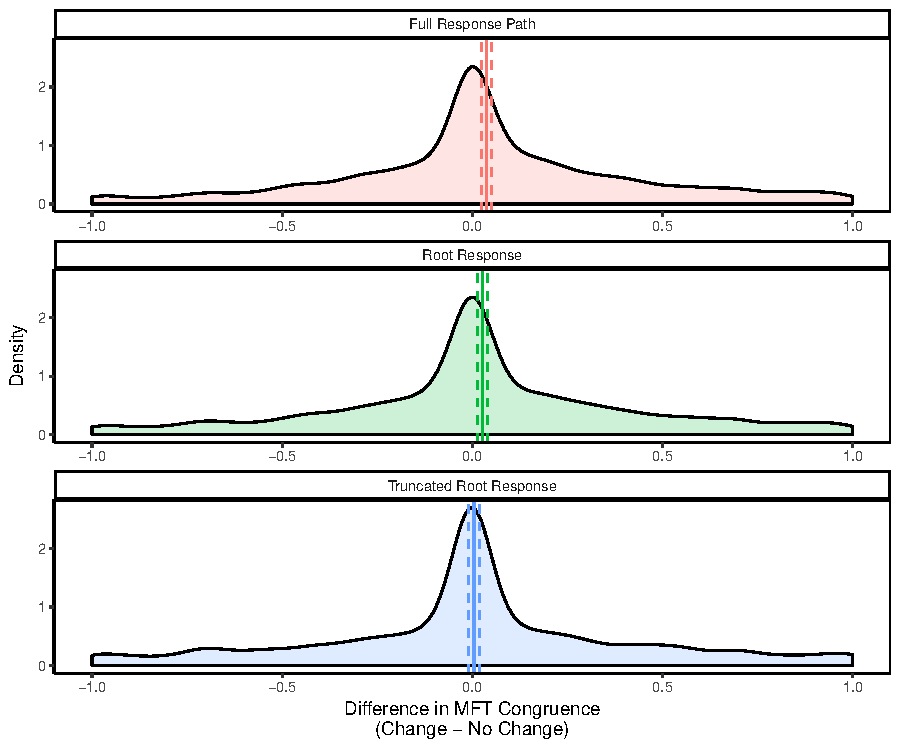
\includegraphics{/data/Dropbox/Uni/Projects/2017/cmv/calc/fig/cosine_density.pdf}
\caption{Distributions of the difference in MFT cosine similarity.}
\end{figure}


\begin{figure}[h]
\centering
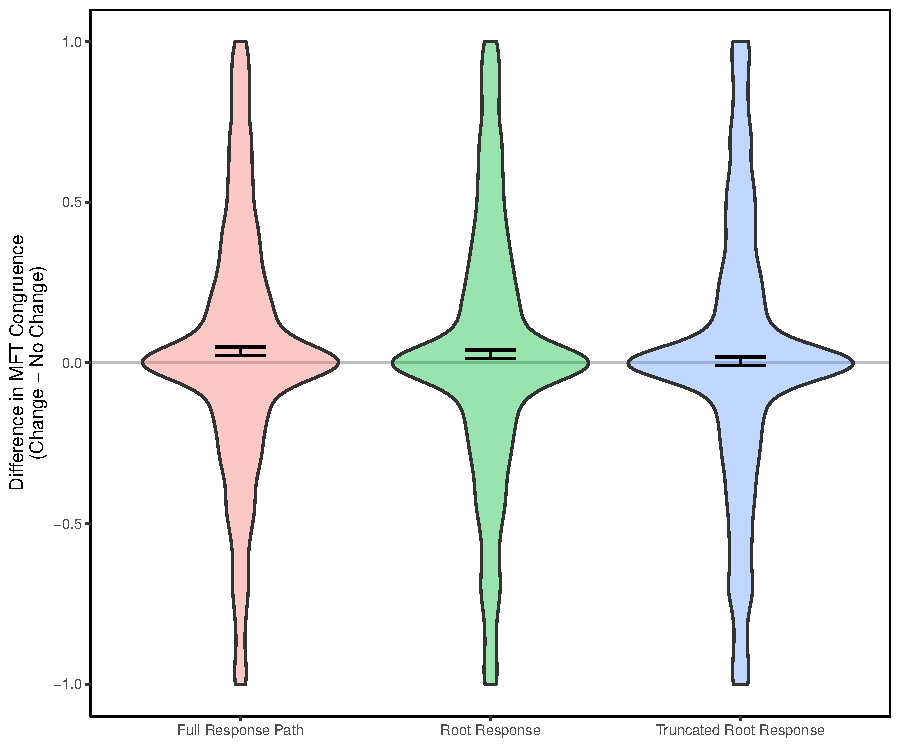
\includegraphics{/data/Dropbox/Uni/Projects/2017/cmv/calc/fig/cosine_violin.pdf}
\caption{Distributions of the difference in MFT cosine similarity (Violin Plot).}
\end{figure}

\clearpage
\section{Structural Topic Model Results}
\renewcommand\thefigure{B.\arabic{figure}}
\renewcommand\thetable{B.\arabic{table}}
\setcounter{figure}{0}
\setcounter{table}{0}

\subsection{Original Posts}

\begin{figure}[h]
\centering
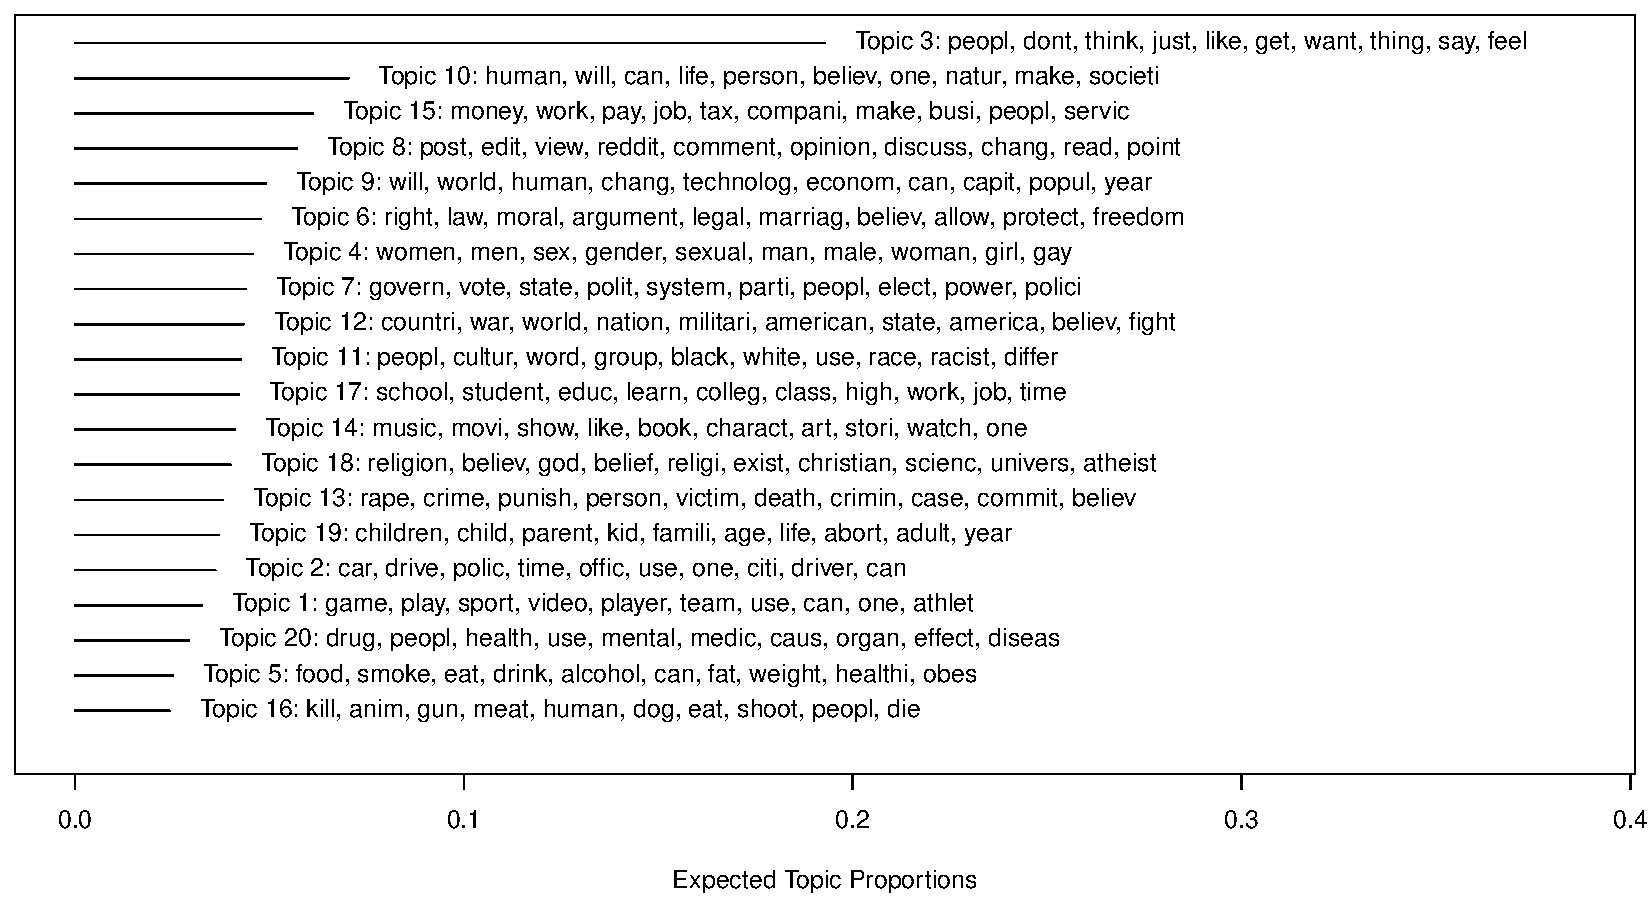
\includegraphics[width=\textwidth]{/data/Dropbox/Uni/Projects/2017/cmv/calc/fig/stm_op_prop.pdf}
\caption{Check description ch. 2}
\end{figure}

\begin{figure}[h]
\centering
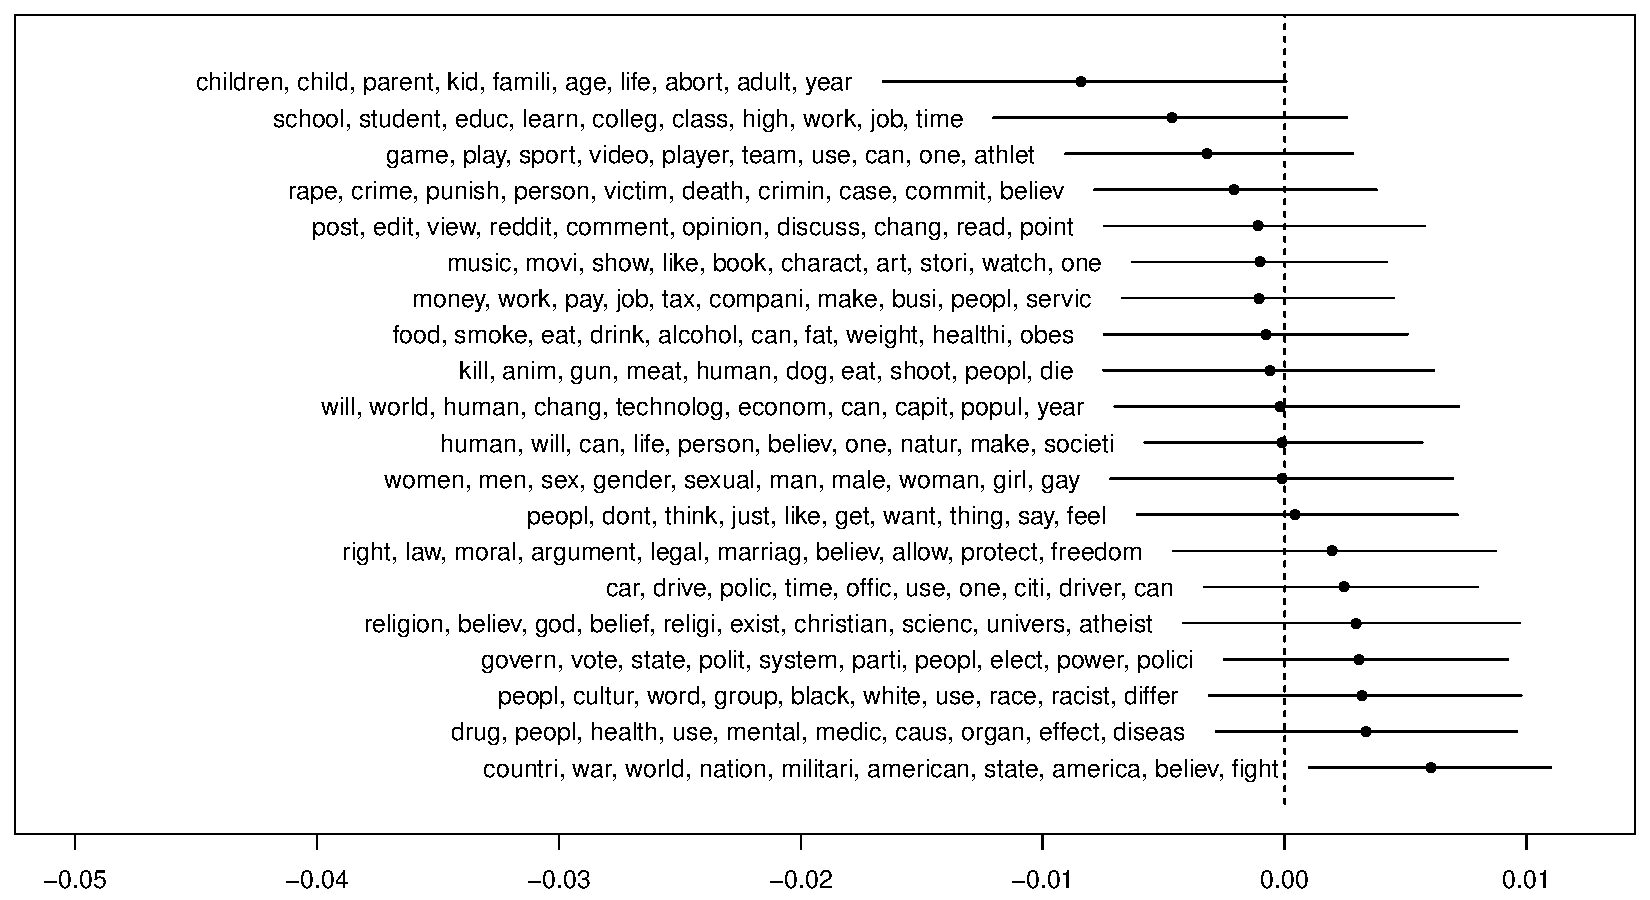
\includegraphics[width=\textwidth]{/data/Dropbox/Uni/Projects/2017/cmv/calc/fig/stm_op_diff.pdf}
\caption{Check description ch. 2}
\end{figure}

\clearpage
\subsection{Responses}

\begin{figure}[h]
\centering
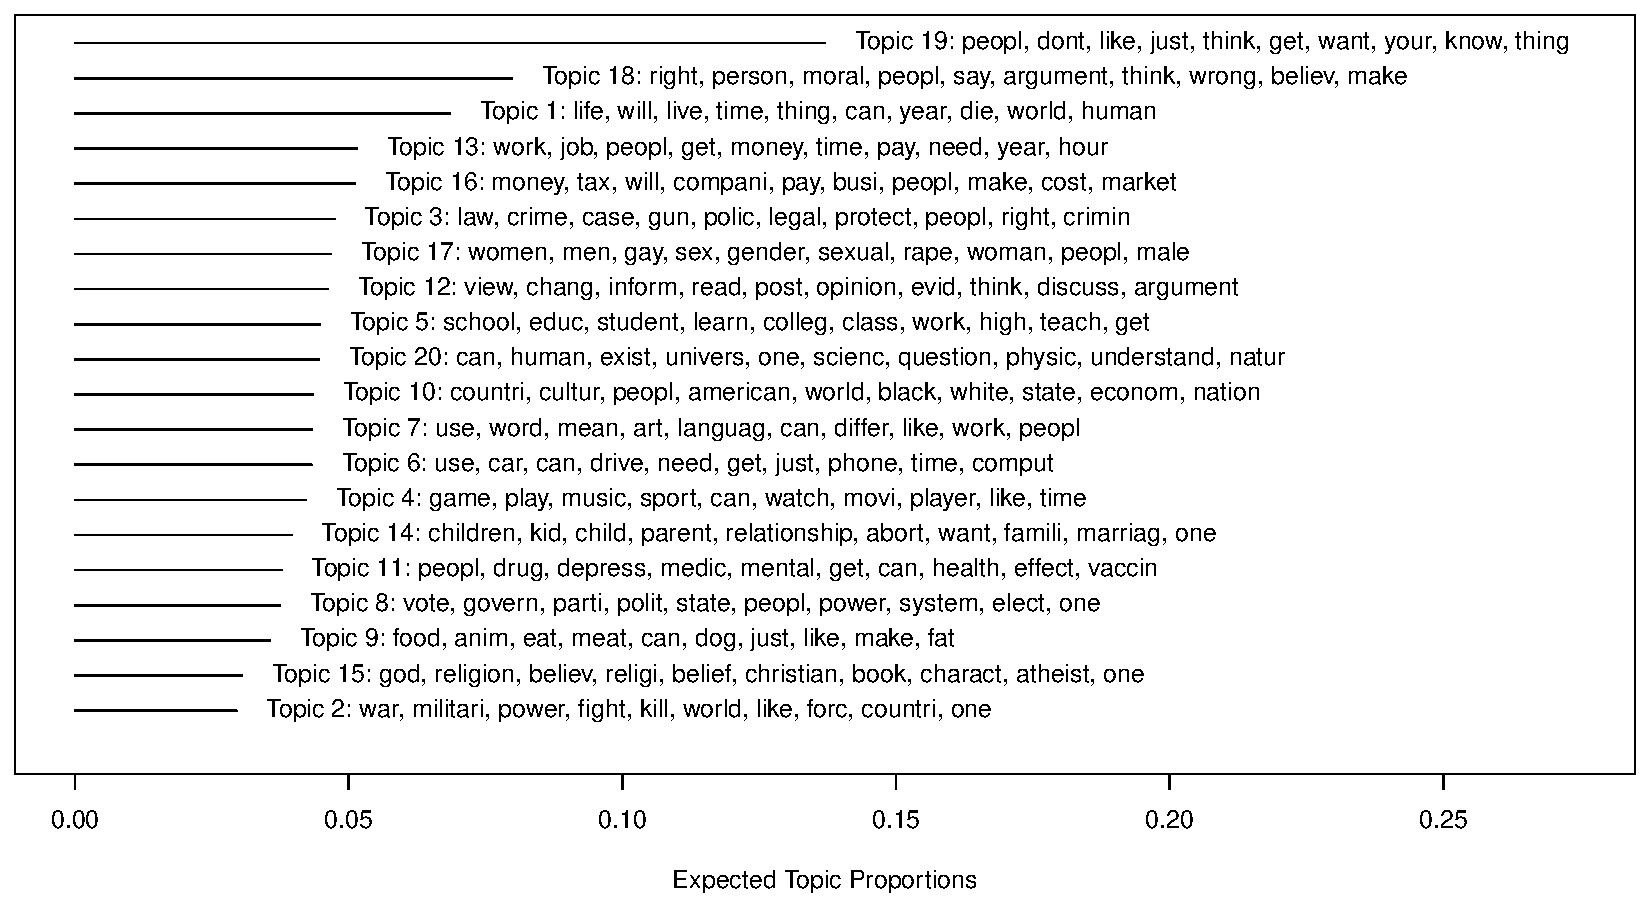
\includegraphics[width=\textwidth]{/data/Dropbox/Uni/Projects/2017/cmv/calc/fig/stm_pair_prop.pdf}
\caption{Check description ch. 2}
\end{figure}

\begin{figure}[h]
\centering
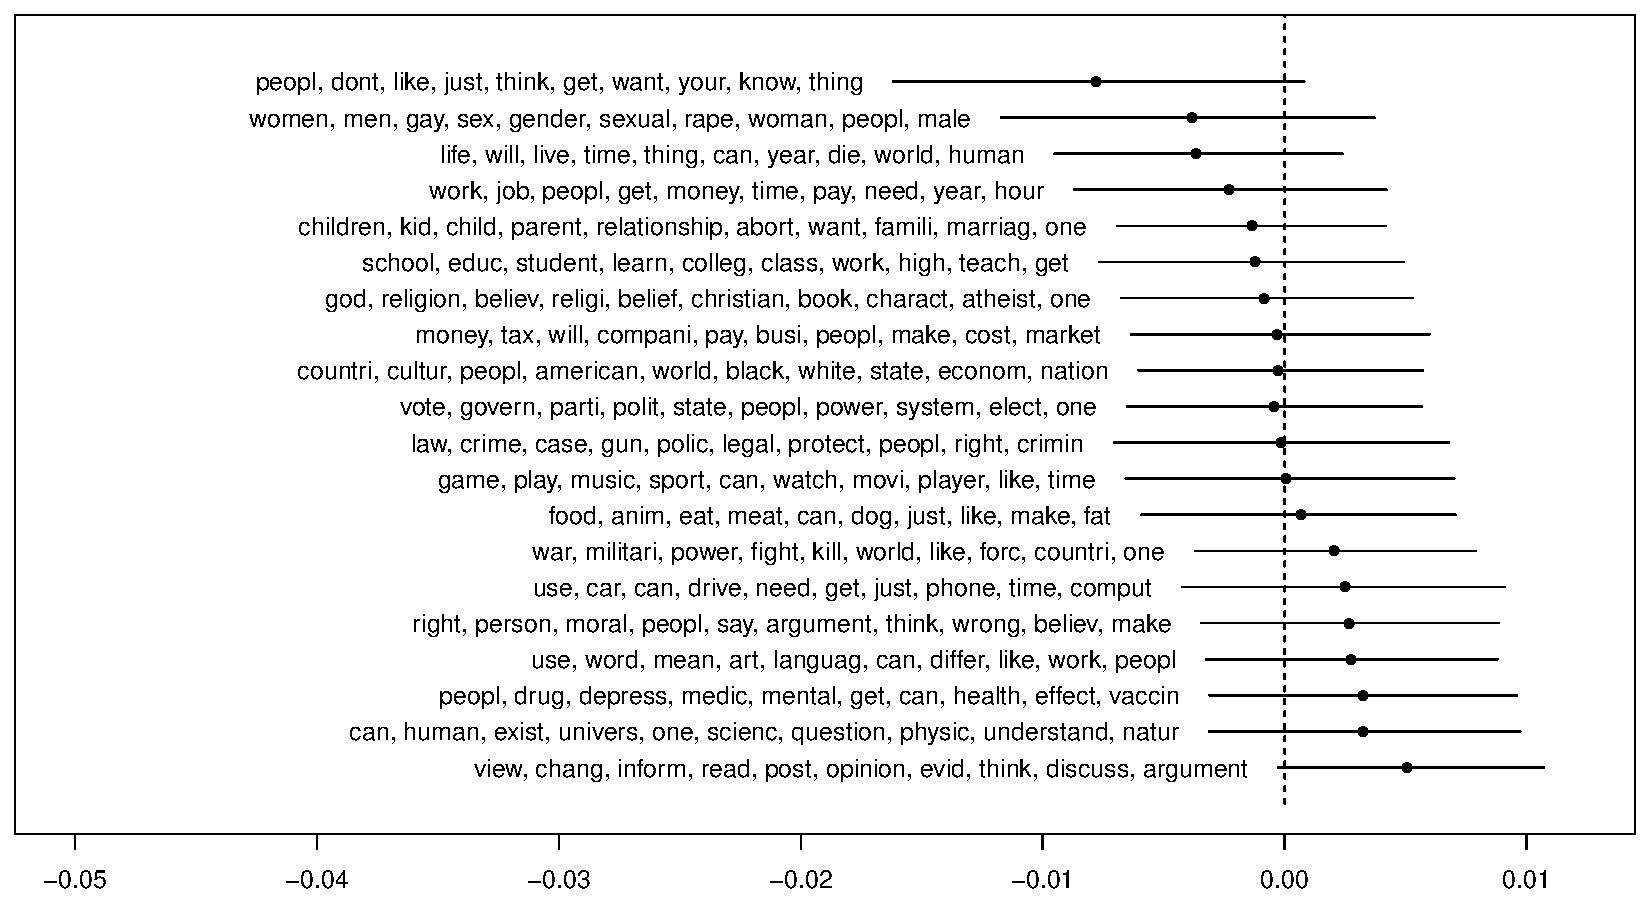
\includegraphics[width=\textwidth]{/data/Dropbox/Uni/Projects/2017/cmv/calc/fig/stm_pair_diff.pdf}
\caption{Check description ch. 2}
\end{figure}

